\documentclass[../../../main]{subfiles}
\begin{document}

\section{原理}
複数の波が1点で出会う時、その点での波の振幅は各波の振幅の和となるが、
位相関係の違いによって合成波の振幅が変化することを干渉という。


図\ref{fig:single_hole_interference}に示すように、一点\( \mathrm{Q} \)より出た光がついたてに立てられた開口\( \mathrm{S} \)を通過し、
スクリーンに当たった状況を考える。
スクリーン上の点 \( \mathrm{M} \) の光の強さを求めるために、Qから出た光が開口Sのふちに達しているとするとき、
半径1のところの波を \( A = A_0 \sin \omega t \)とすれば、波面 \( \mathrm{E} \) 上では、
\begin{equation}
	A = A_0 \sin \left( \omega t - \dfrac{2\pi}{\lambda} a  \right)
\end{equation}
と書ける。
\( \overline{\mathrm{PM}} \) を\( r \)とおくと、Pにおける微小面積 \( \odif{e} \)から出た光のMにおける振幅は、
\begin{equation}
	A = \dfrac{\alpha}{r} \dfrac{A_0}{a} \sin \left[ \omega t - \dfrac{2\pi}{\lambda} \left( a+r \right)  \right]
\end{equation}
と表せる。
ただし、 \( \alpha \) は光の方向に関係する量であるが、ここでは \( \alpha = 1 \) とする。

Mにおける振幅は開口S全体にわたる積分で求められるから、
\begin{equation}
	A(M) = \int_{E} \dfrac{A_0}{ar} \sin  \left[ \omega t - \dfrac{2\pi}{\lambda} \left( a + r \right)  \right] \odif{e}
\end{equation}
\( \dfrac{A_0}{ar} \approx \dfrac{A_0}{ab} \left( \because b \sim r \right)  \)として、さらに振幅比のみを考えて、
\( \dfrac{A_0}{ab} = 1  \) とする。

簡単のため2次元で考えると、 \( \mathrm{Q'} \) を原点とし、 \( \mathrm{OQ'} \) に直角に紙面内で\( x \)軸をとり、P, Mの座標を \( \mathrm{P}(\xi, -b + \zeta) \), \( \mathrm{M}(x, 0) \) とすると、
\begin{equation}\label{eq:single_hole_interference_r}
	r = \sqrt{\left( \xi - x \right)^2 + \left( b - \zeta \right)^2 }
\end{equation}
波面の式を
\begin{equation}\label{eq:single_hole_interference_wave_surface}
	\xi^2 + \left( a + \zeta \right)^2 = a^2
\end{equation}
とすると、\ref{eq:single_hole_interference_r}式は
\begin{align}\label{eq:single_hole_interference_r_2}
	r & = \sqrt{\xi^2 - 2x\xi+x^2 + b^2 - 2b\zeta + \zeta^2} \nonumber \\
	  & = \sqrt{x^2 + b^2 - 2 \left( a + b \right) \zeta - 2x \xi}.
\end{align}
いま、 \( \zeta \) が \( a,b \) に比べ十分小さいとして、\( \zeta^2 \)以上の項を無視すると、
\ref{eq:single_hole_interference_wave_surface}式は
\begin{equation}
	\zeta = - \dfrac{\xi^2}{2a}
\end{equation}
これを\ref{eq:single_hole_interference_r_2}に代入して、
\begin{equation}\label{eq:sigle_hole_interference_r_taylor}
	r = b \left( 1 + \dfrac{x^2}{2b^2}  \right) - \left( \dfrac{x \xi}{b} - \dfrac{a+b}{2ab}\xi^2   \right) + \cdots = \overline{\epsilon} + \epsilon(\xi)
\end{equation}
ただし、 \( \overline{\epsilon} \) は \( \xi \) に依存しない項、 \( \epsilon(\xi) \) は \( \xi \) の関数とする。
これより、
\begin{align}\label{eq:single_hole_interference_amplitude}
	A(M) & = \int_E \sin \left[ \omega t - \dfrac{2\pi}{\gamma} \left( a + \overline{\epsilon} + \epsilon \right)  \right] \odif{e} \nonumber                                                               \\
	     & = C \sin \left[ \omega t - \dfrac{2\pi}{\lambda} \left( a + \overline{\epsilon} \right)  \right] + S \cos \left[ \omega t - \dfrac{2\pi}{\lambda} \left( a + \overline{\epsilon} \right) \right]
\end{align}
ただし、
\begin{equation}
	\begin{aligned}
		C & = \int_E \cos \dfrac{2\pi}{\lambda} \left( \dfrac{x \xi}{b} - \dfrac{a+b}{2ab} \xi^2   \right) \odif{e} \\
		S & = \int_E \sin \dfrac{2\pi}{\lambda} \left( \dfrac{x \xi}{b} - \dfrac{a+b}{2ab} \xi^2   \right) \odif{e}
	\end{aligned}
\end{equation}
が得られる。
強度は \( |A|^2 = C^2 + S^2 \) で与えられる。

次に、共役面の回折像について考える。開口Sの前にレンズLがあり、 \( \mathrm{Q'} \) が\( Q \)の幾何工学的像である場合、
積分すべき波面はQより発散するか、\( \mathrm{Q'} \)へ収束する球面であるから、図\ref{fig:single_hole_interference_2}のように、
後者をとり、 \( \mathrm{Q'} \) を中心とする半径\( b \)の球面 \( \mathrm{E'} \) とする。
光源から波面 \( \mathrm{E'} \) 上の一点までの光路長はすべて等しく、これを \( a \), \( \overline{\mathrm{PM}} = r \) とすれば、
波面の式は、 \( \xi^2 + \left( b - \zeta \right)^2 = b^2 \) であるので、
\begin{align}
	a + r & = a + b + (r - b)                                                                            \nonumber \\
	      & = a + b + \left( \sqrt{ \left( \xi - x \right)^2 + \left( b - \zeta \right)^2 } - b  \right) \nonumber \\
	      & \approx \left( a + b + \dfrac{x^2}{2b}  \right) - \dfrac{x \xi}{b}
\end{align}
第一項は、 \( \xi \) を含まず位相のみに関係し、強度の積分に関係ないから\ref{eq:sigle_hole_interference_r_taylor}式の \( \overline{\epsilon} \) に相当し、
\begin{equation}
	\epsilon = \dfrac{2\pi}{\lambda} \dfrac{x \xi}{b} = kx \xi \quad \left(k = \dfrac{2\pi}{\lambda b}\right)
\end{equation}
となるから、\ref{eq:single_hole_interference_amplitude}式は、
\begin{equation}
	\begin{aligned}
		C      & = \int_E \cos \left( kx \xi \right) \odif{\xi}  \\
		S      & = \int_E \sin \left( kx \xi \right) \odif{\xi}  \\
		C + iS & = \int_E \exp \left( ikx \xi \right) \odif{\xi}
	\end{aligned}
\end{equation}
とかける。

3次元の場合も同様にして、P,Mの座標を \( (\xi, \eta, b - \xi) \), \( (x, y, 0) \) として、
\begin{equation}
	\begin{aligned}
		C & = \iint  \cos k \left( x \xi + y \eta \right) \odif{\xi} \odif{\eta} \\
		S & = \iint  \sin k \left( x \xi + y \eta \right) \odif{\xi} \odif{\eta}
	\end{aligned}
\end{equation}
を得る。

以上の式から、この回折は開口Sのフーリエ変換によって与えられることがわかる。

\begin{figure}[htbp]\centering
	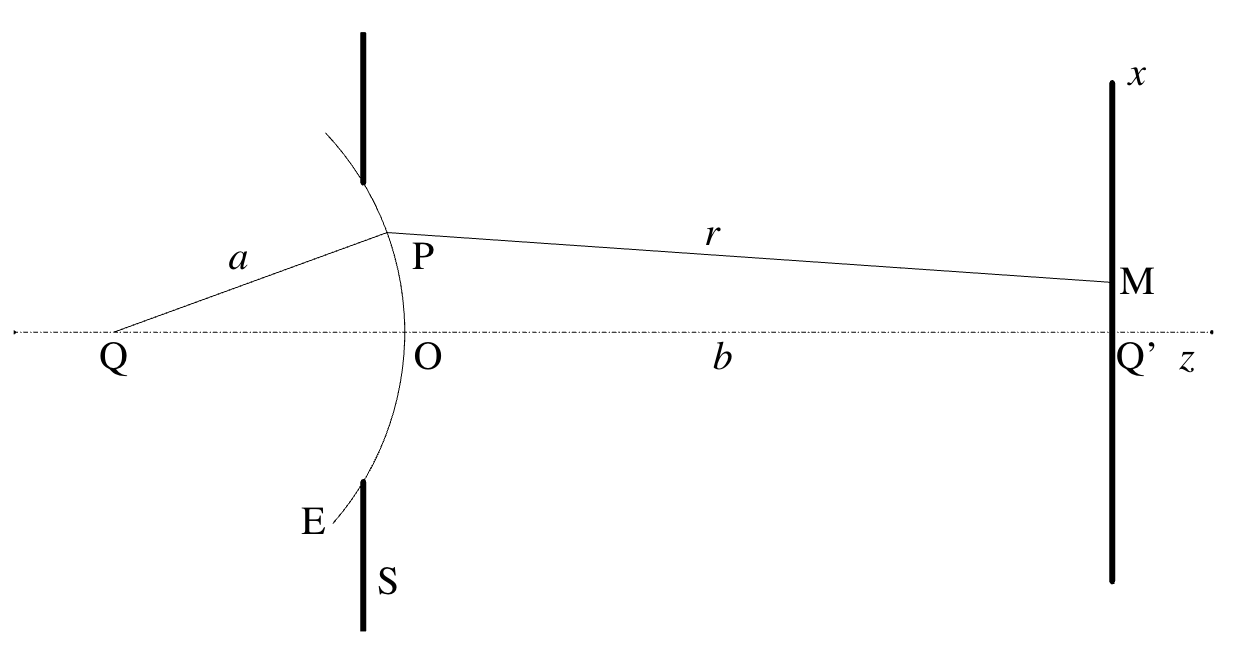
\includegraphics[width=\linewidth]{src/figures/principle/single_hole.png}
	\caption{開口Sによる光源Qの回折}
	\label{fig:single_hole_interference}
\end{figure}

\begin{figure}[htbp]\centering
	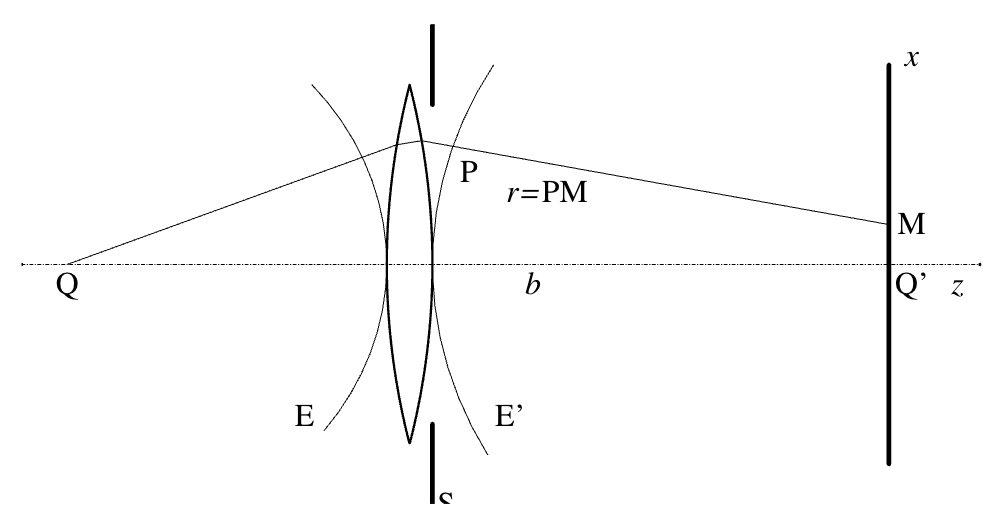
\includegraphics[width=\linewidth]{src/figures/principle/single_hole_2.png}
	\caption{光源Qのフラウンホーファー回折像}
	\label{fig:single_hole_interference_2}
\end{figure}


% \subsection{Young's Interference}
% Fig.\ref{fig:young_interference}に示すように一つの光源から出た光が2つのスリットを通過し、
% 光束に垂直におかれ微小距離 \( d \) を隔て互いに平行なスリット \( \mathrm{S_1}, \mathrm{S_2} \) によって2つの光路に分かれ、
% スクリーン上の 点\( P \)  に到達した場合に、2つの光の位相が \( \delta \) だけずれているとすると、
% \begin{equation}\label{eq:young_interference_phase_difference}
%     \delta = \dfrac{2\pi}{\lambda}\left( \overline{\mathrm{S_2P}} - \overline{\mathrm{S_1P}} \right)
% \end{equation}
% 成分波の振幅が\( a \)とすると、強度\( I \)は
% \begin{equation}
%     I \sim 4 a ^2 \cos ^2 \dfrac{\delta}{2}
% \end{equation}
% と表される。
% また、\ref{eq:young_interference_phase_difference}式で
% \( \overline{\mathrm{S_1P}} = \sqrt{D ^2 + \left( x + \dfrac{d}{2}  \right) ^2} \)、
% \( \overline{\mathrm{S_2P}} = \sqrt{D ^2 + \left( x - \dfrac{d}{2}  \right) ^2} \)とすると、
% より、 \( d \ll D \) として
% \begin{align}\label{eq:young_interference_phase_difference_approx}
%     \overline{S_2P} - \overline{S_1P} & = \sqrt{D ^2 + \left( x - \dfrac{d}{2}  \right) ^2} - \sqrt{D ^2 + \left( x + \dfrac{d}{2}  \right) ^2}                                                                                 \nonumber  \\
%                                       & = D \left\{ \left( 1 + \left( \frac{x+\frac{d}{2}}{D}  \right) ^2  \right) ^{\frac{1}{2} } - \left( 1 - \left( \dfrac{x-\frac{d}{2}}{D}  \right)^{2}  \right) ^{\frac{1}{2} }   \right\} \nonumber \\
%                                       & \simeq \dfrac{D}{2}  \left\{ \left( \dfrac{x+\frac{d}{2}}{D}  \right) ^2 - \left( \dfrac{x-\frac{d}{2}}{D}  \right) ^2  \right\} \nonumber                                                         \\
%                                       & = \dfrac{d}{D} x \nonumber                                                                                                                                                                         \\
%     \therefore \delta                 & = \dfrac{2\pi}{\lambda} \dfrac{d}{D} x.
% \end{align}
% スクリーン上で干渉光の強度が最大となるのは、
% \begin{align}
%     \delta & = 2n\pi \quad (n = 0, 1, 2, \cdots) \nonumber \\
%     x      & = n \lambda \dfrac{D}{d}
% \end{align}
% のときで強度が \( 4a \) となる。

% \begin{figure}[htbp]
	\centering
	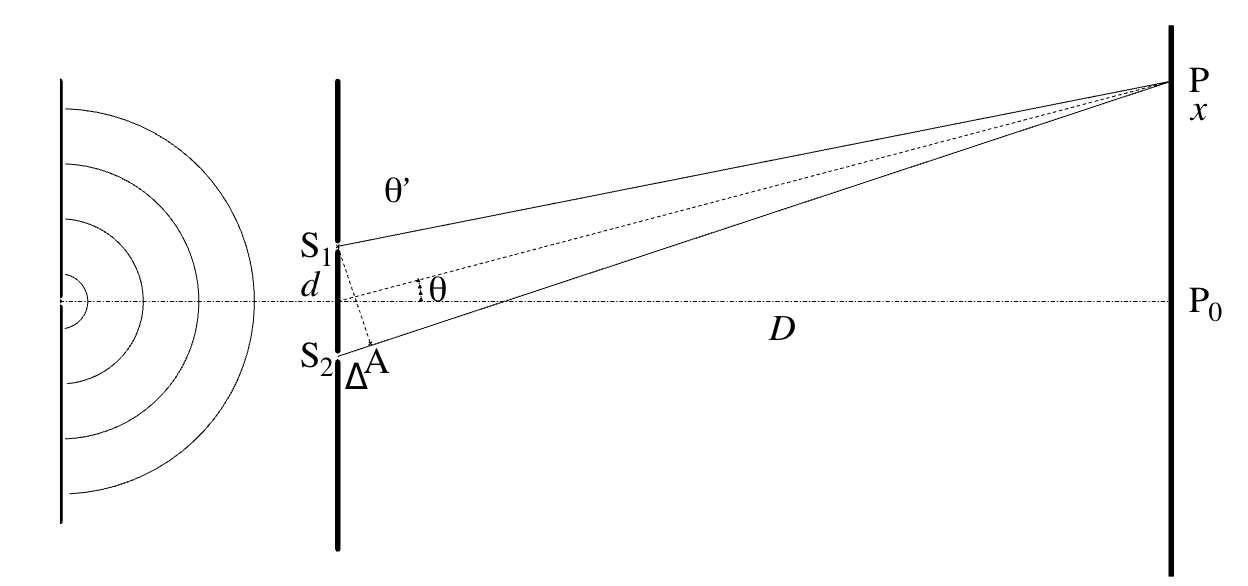
\includegraphics[width=\linewidth]{src/figures/principle/young_interference.png}
	\caption{Youngの干渉実験の概念図}\label{fig:young_interference}
\end{figure}


% \subsection{フラウンホーファー回折}
% \begin{figure}[htbp]\centering
	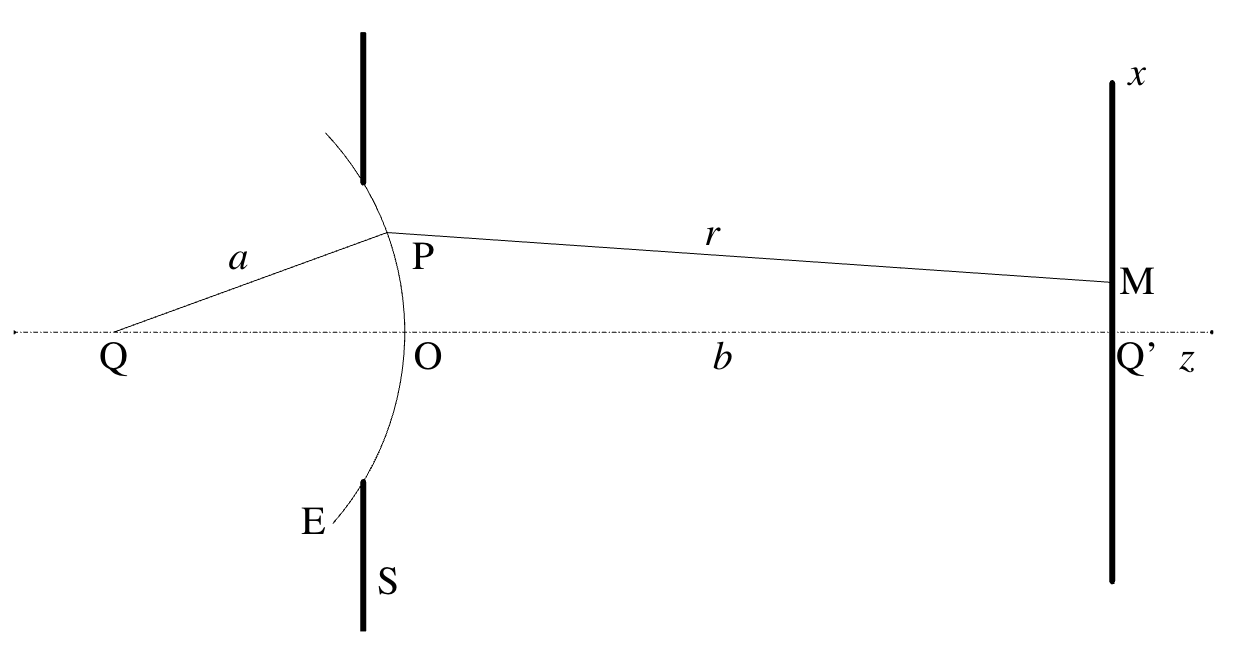
\includegraphics[width=\linewidth]{src/figures/principle/single_hole.png}
	\caption{開口Sによる光源Qの回折}
	\label{fig:single_hole_interference}
\end{figure}


\end{document}
